%==============================================================================
%== template for LATEX poster =================================================
%==============================================================================
%
%--A0 beamer slide-------------------------------------------------------------
\documentclass[final]{beamer}

\usepackage[orientation=landscape,
            scale=1.05         % font scale factor
           ]{beamerposter}
\geometry{papersize={60in,36in}}
\usepackage[numbers,square]{natbib}
\renewcommand{\bibsection}{\subsubsection*{\bibname } } % eliminates the unwanted bibliography section head
\renewcommand{\newblock}{}
\bibliographystyle{abbrvnat}


%\setlength{\paperwidth}{33.1in}
%\setlength{\paperheight}{23.4in}
\setlength{\paperwidth}{60in}
\setlength{\paperheight}{36in}
           
\geometry{
  hmargin=2.5cm, % little modification of margins
}


%
\usepackage[utf8]{inputenc}

\linespread{1.15}
%
%==The poster style============================================================
\usetheme{sharelatex}

%==Title, date and authors of the poster=======================================
\title
[American Geophysical Union Annual Meeting. San Francisco, CA. December
12-16, 2016.] % Conference
{ % Poster title
Distilling Design Patterns From Agile Curation Case Studies (IN41A-1656)
}

\author{ % Authors
Karl Benedict\inst{1} \and W. Christopher Lenhardt\inst{2} \and Joshua Young\inst{3}}

\institute{
\inst{1} University of New Mexico
\inst{2} Renaissance Computing Institute
\inst{3} University Corporation for Atmospheric Research
}


\date{December 15, 2016}



\begin{document}
\begin{frame}[t]
%==============================================================================
\begin{multicols}{3}

%--abstract-------------------------------------------------------------

\subsection{Abstract}

In previous work the authors have argued that there is a need to take a
new look at the data management lifecycle. Our core argument is that the
data management lifecycle needs to be in essence deconstructed and
rebuilt. As part of this process we also argue that much can be gained
from applying ideas, concepts, and principles from agile software
development methods. To be sure we are not arguing for a rote
application of these agile software approaches, however, given various
trends related to data and technology, it is imperative to update our
thinking about how to approach the data management lifecycle, recognize
differing project scales, corresponding variations in structure, and
alternative models for solving the problems of scientific data curation.
In this paper we will describe what we term agile curation design
patterns, borrowing the concept of design patterns from the software
world and we will present some initial thoughts on agile curation design
patterns as informed by a sample of data curation case studies solicited
from participants in agile data curation meeting sessions conducted in
2015-16.

%--End of abstract------------------------------------------------------




%==============================================================================
%==The poster content==========================================================
%==============================================================================

\section{Introduction}\label{introduction}

The challenges that must be addressed by current research data
management and curation processes and strategies consist of a
combination of established practices that are not compatible with
increasing complexity in the data management landscape at the project
level; increasing expectations by sponsors, publishers, and institutions
relating to data management and curation; and rapid growth in the
volume, variety and velocity (three dimensions commonly used to define
``big data'') of data generated by and used in research. In combination
these challenges translate into an increasing need to develop effective
data management and curation strategies that align with a set of
\emph{shared values and principles} that inform management and curation
objectives, and implement processes that are \emph{well documented and
portable} across specific data management projects. It is this latter
requirement that is addressed in this poster - the development of a
framework for capturing elements of successful data curation activities
and generalizing those elements into linkages with existing design
patterns, or defining new design patterns when they don't exist.

\subsection{Work to Date}\label{work-to-date}

Thus far the focus of the project's work has been on developing a
framework within which the team can discuss the concept of \emph{agile
data curation} with the community, and iteratively evolving that
framework through a series of meeting sessions, workshops and
presentations that have been given at multiple venues including AGU
(2014, 2015), ESIP Federation Meeting (2016), Research Data Alliance
(2014, 2015, 2016), and SciDataCon (2016). In these various activities
the team has worked on communicating the conceptual framework for our
vision of agile data curation, presented a variety of initial values and
principles derived from those defined in the \emph{Manifesto for Agile
Software Development} \citep{beck_manifesto_2001}, and solicited the
presentation of data management projects that exemplify (either
intentionally or unintentionally) these principles.

\section{Conceptual Model for Agile Data Curation Design
Patterns}\label{conceptual-model-for-agile-data-curation-design-patterns}

While this outreach and community engagement work described above is
continuing, the work presented here is the starting point for our third
goal of adapting the concept of design patterns that had been developed
for object oriented software development \citep{gamma_design_1995}, and
extended into related domains
\citep{daigneau_service_2011, lasater_design_2010, ackerman_patterns-based_2010, schwinn_design_2005, hohpe_enterprise_2003},
for use in documenting \emph{named} data curation \emph{problems},
\emph{solutions}, and \emph{consequences} that provide
\emph{descriptions of generalized data components that are customized to
solve a general design problem in a particular context} (adapted from
\citep[section 1.1]{gamma_design_1995}).

The conceptual model that the research team has developed for mapping
research data curation functional requirements into design patterns
represents a combination of specific research activities that have
data-related components (as exemplified in Figure 1) and linkages
between those components as envisioned by a model such as the \emph{Open
Archival Information System} (OAIS -
\citep{book_reference_2012, _iso_2012, oclc_open_2014} - Figure 2). In
particular, the research team is currently developing a model for
collecting and synthesizing data curation case studies that can be used
as exemplars for identifying existing design patterns or developing new
ones that are relevant in data curation.

\section{Illustration of the Design Pattern Conceptual Model to a
Developed Data Management, Discovery and Access Platform -
GSToRE}\label{illustration-of-the-design-pattern-conceptual-model-to-a-developed-data-management-discovery-and-access-platform---gstore}

The Geographic Storage, Transformation and Retrieval Engine (GSToRE
\citep{_gstore_2016}) is a data management, discovery and access
platform that was developed by the Earth Data Analysis Center as a
tiered services oriented architecture (SOA - Figure 3) that was
developed to meet the needs of multiple research data discovery, access
and interaction models. While the GSToRE platform was not explicitly
developed with any specific design patterns, there are a number of
design patterns that are roughly represented within its design. The
capabilities developed in GSToRE and related research and data
managements steps are linked to each other in the diagram provided in
Figure 3.

\vfill\columnbreak

\begin{figure}[htbp]
\centering
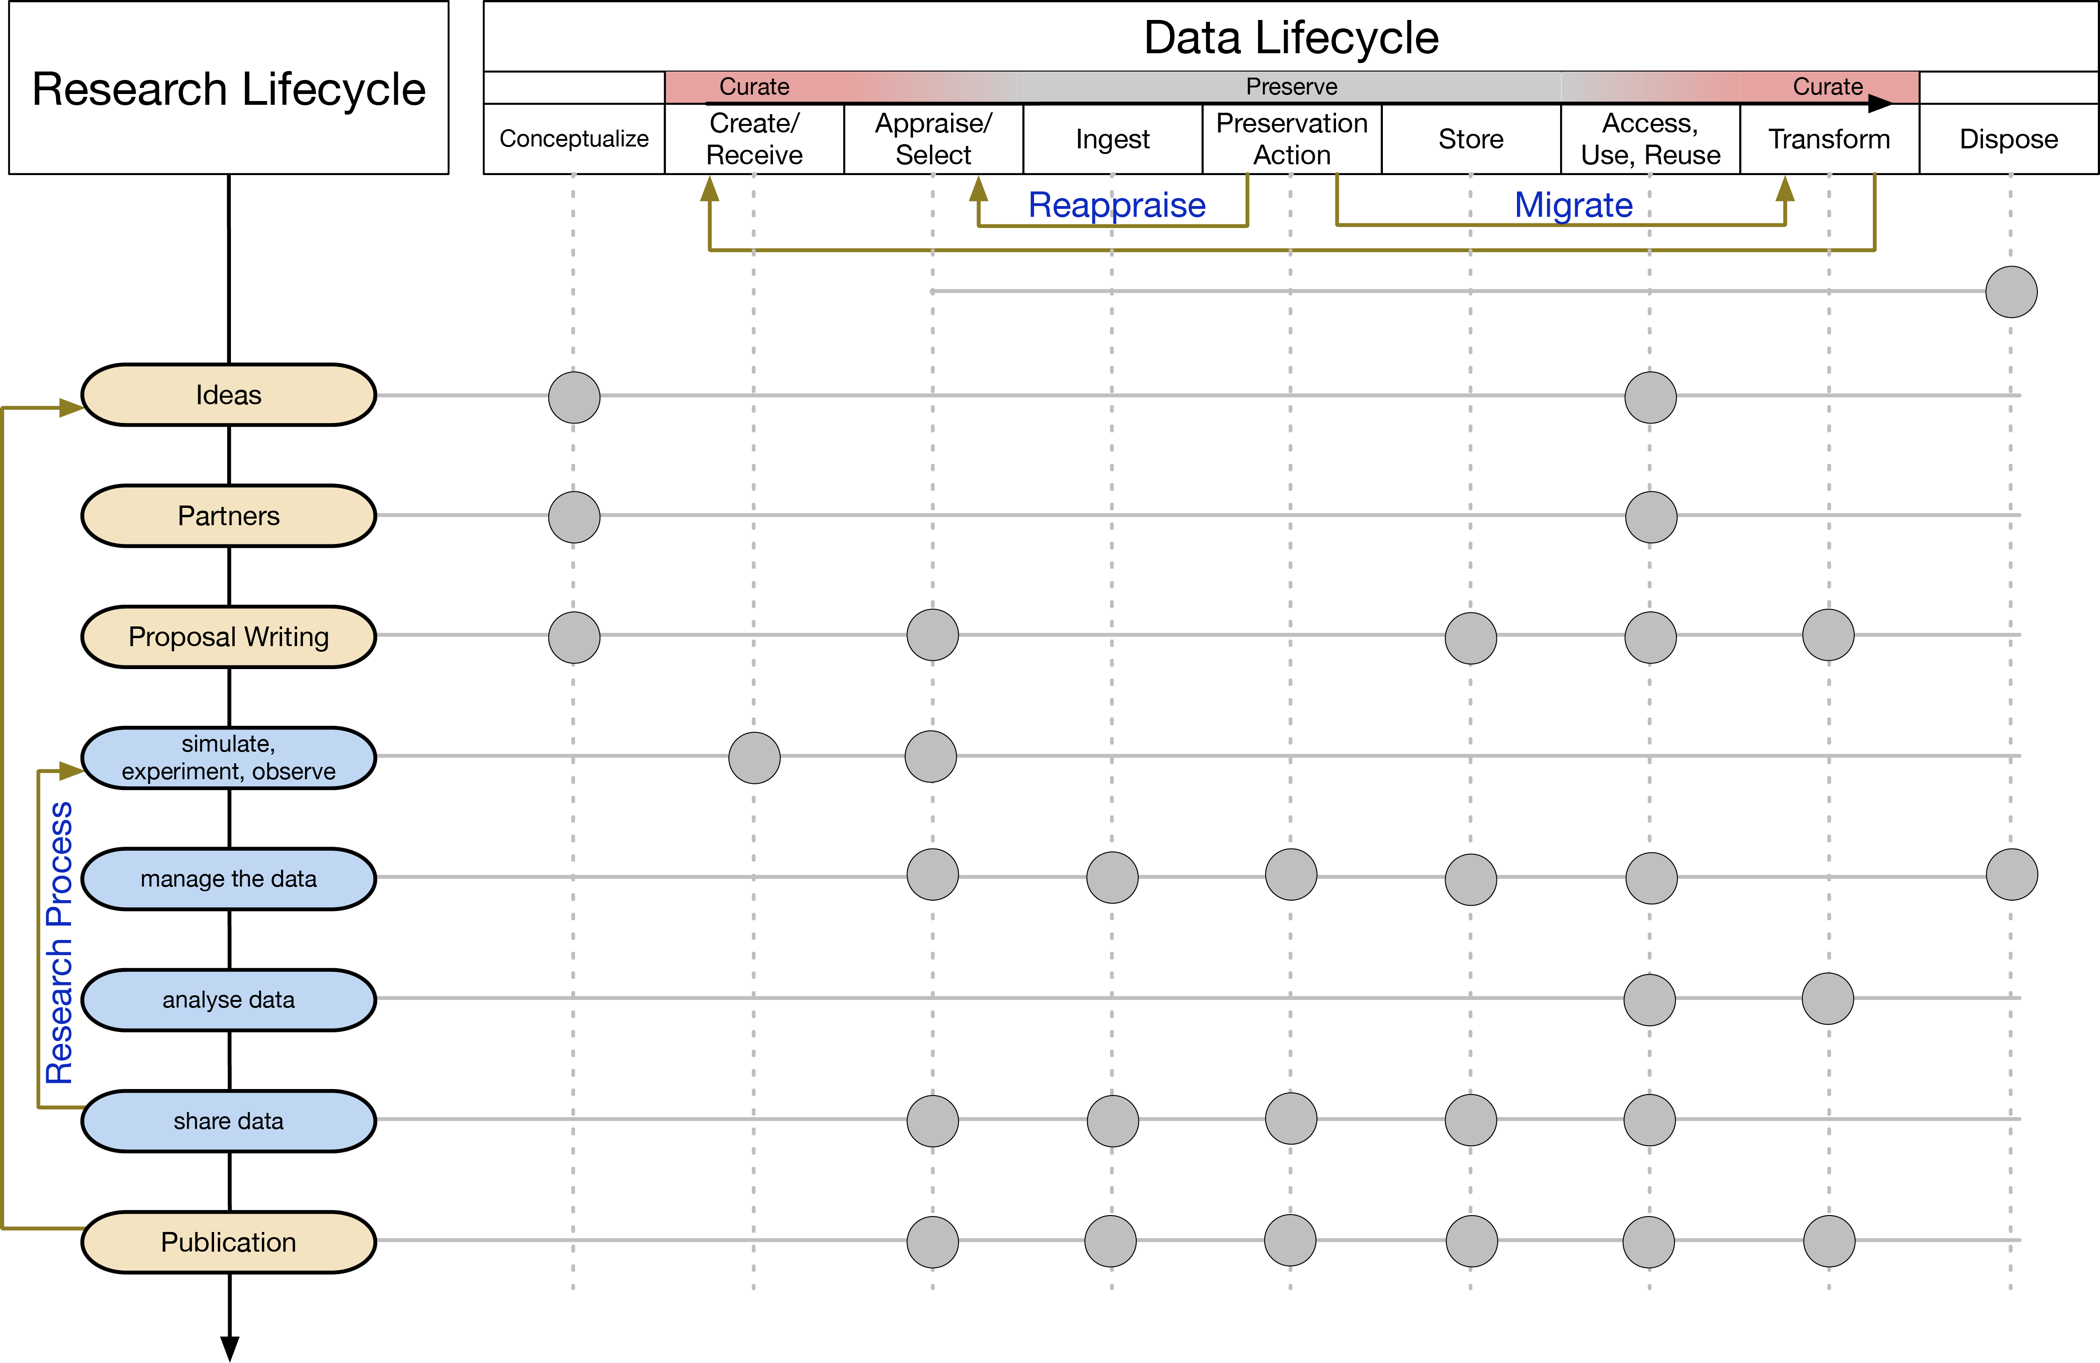
\includegraphics[width=14.00000in]{Research-DataLifecycleIntegration.png}
\caption{Intersection of Research Lifecycle \citep{_how_2014} and Data
Curation Lifecycle Actions \citep{digital_curation_centre_dcc_dcc_nd}
illustrating high-level research activities that involve data-related
functions.}
\end{figure}

\begin{figure}[htbp]
\centering
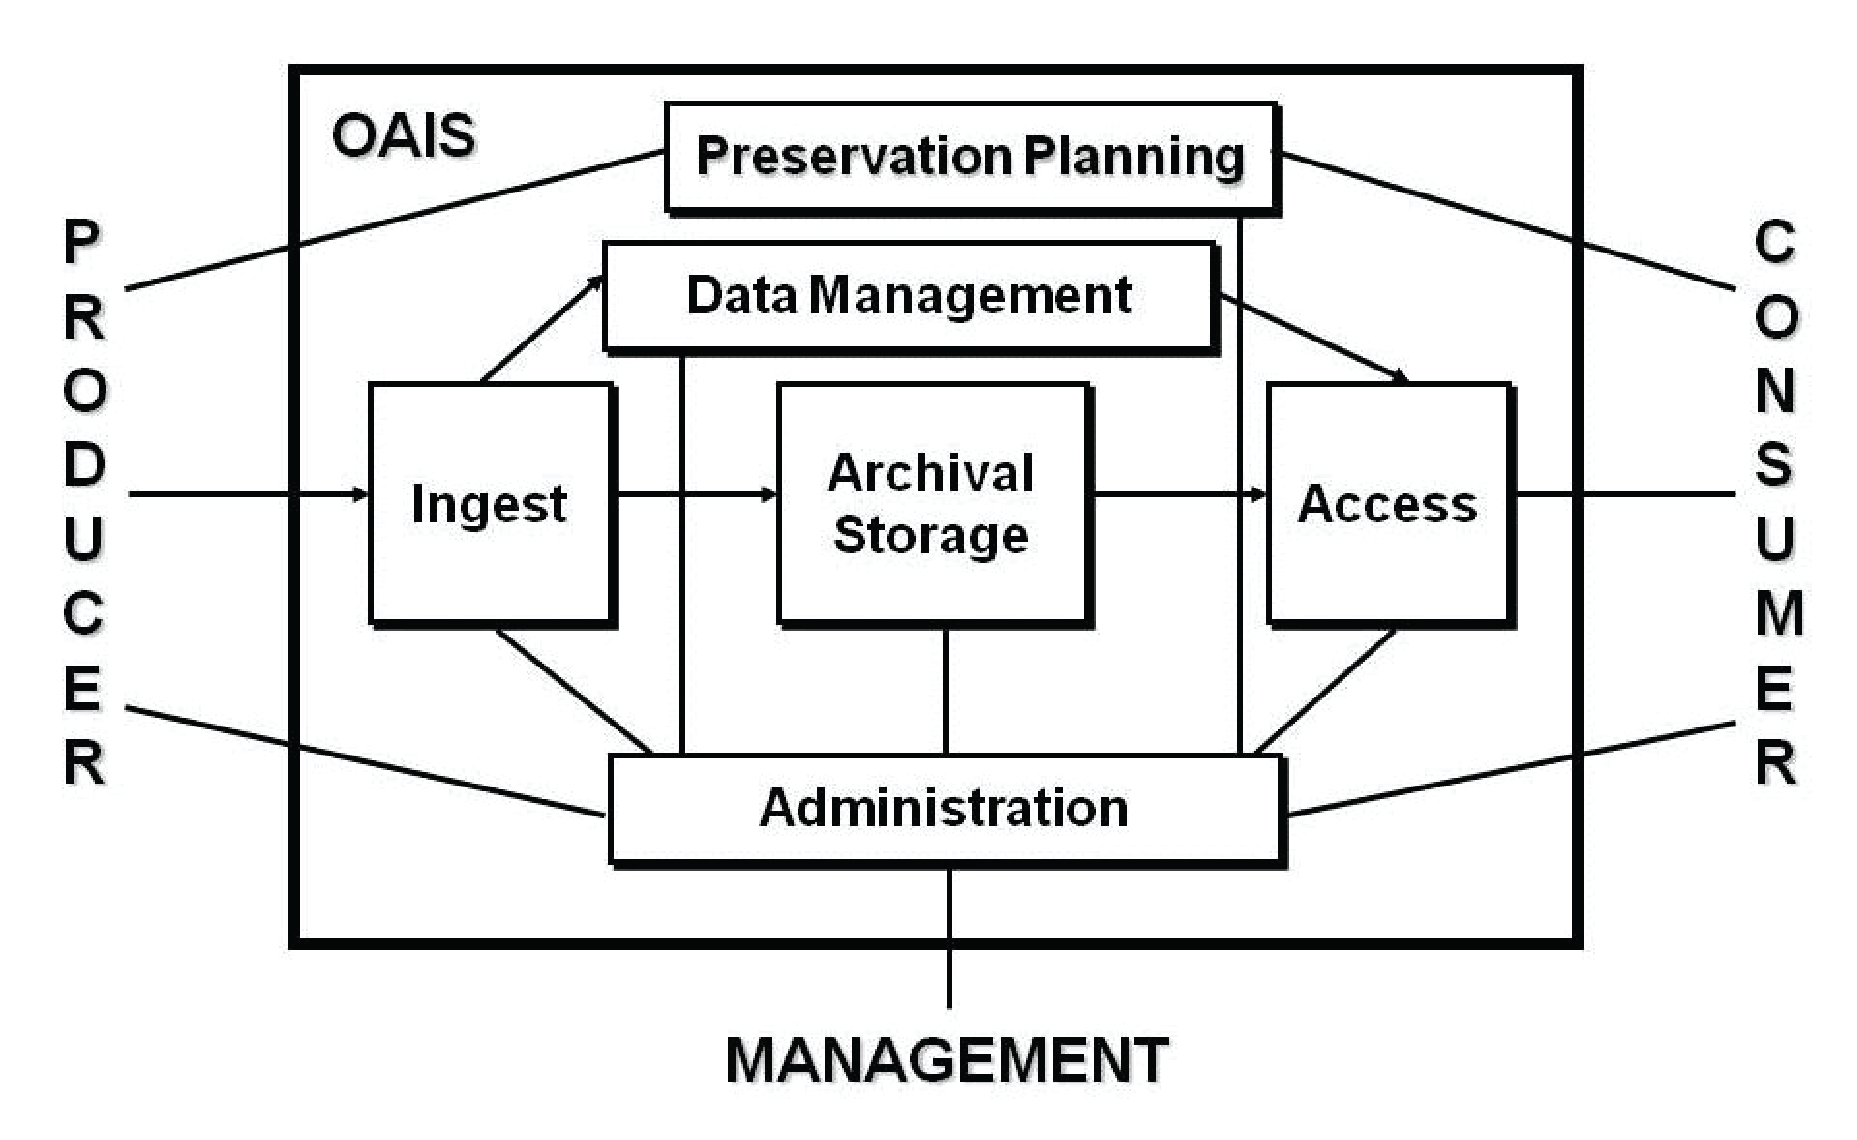
\includegraphics[width=14.00000in]{OAIS_functionalModel.png}
\caption{OAIS Reference Model
\citep{book_reference_2012, _iso_2012, oclc_open_2014} as a high level
interaction model between functional components of a preservation
system}
\end{figure}

\section{Conclusions}\label{conclusions}

While the research team is in the early stages of the identification of
data curation design patterns as part of a larger program of defining an
\emph{agile data curation} approach to research data management and
preservation, the work presented here represents our first attempt to
map an existing data management platform into a set of design patterns
that were developed in support of object oriented software development.
This mapping provides a frame of reference for engaging with the
research data management community in developing a community-based
process for documenting design patterns that have proven effective in
multiple contexts and implementations.

\subsection{Acknowledgements}\label{acknowledgements}

This work has been partially supported through funding from the National
Science Foundation (Award no. IIA-1301346)

\vfill\columnbreak

\begin{figure}[htbp]
\centering
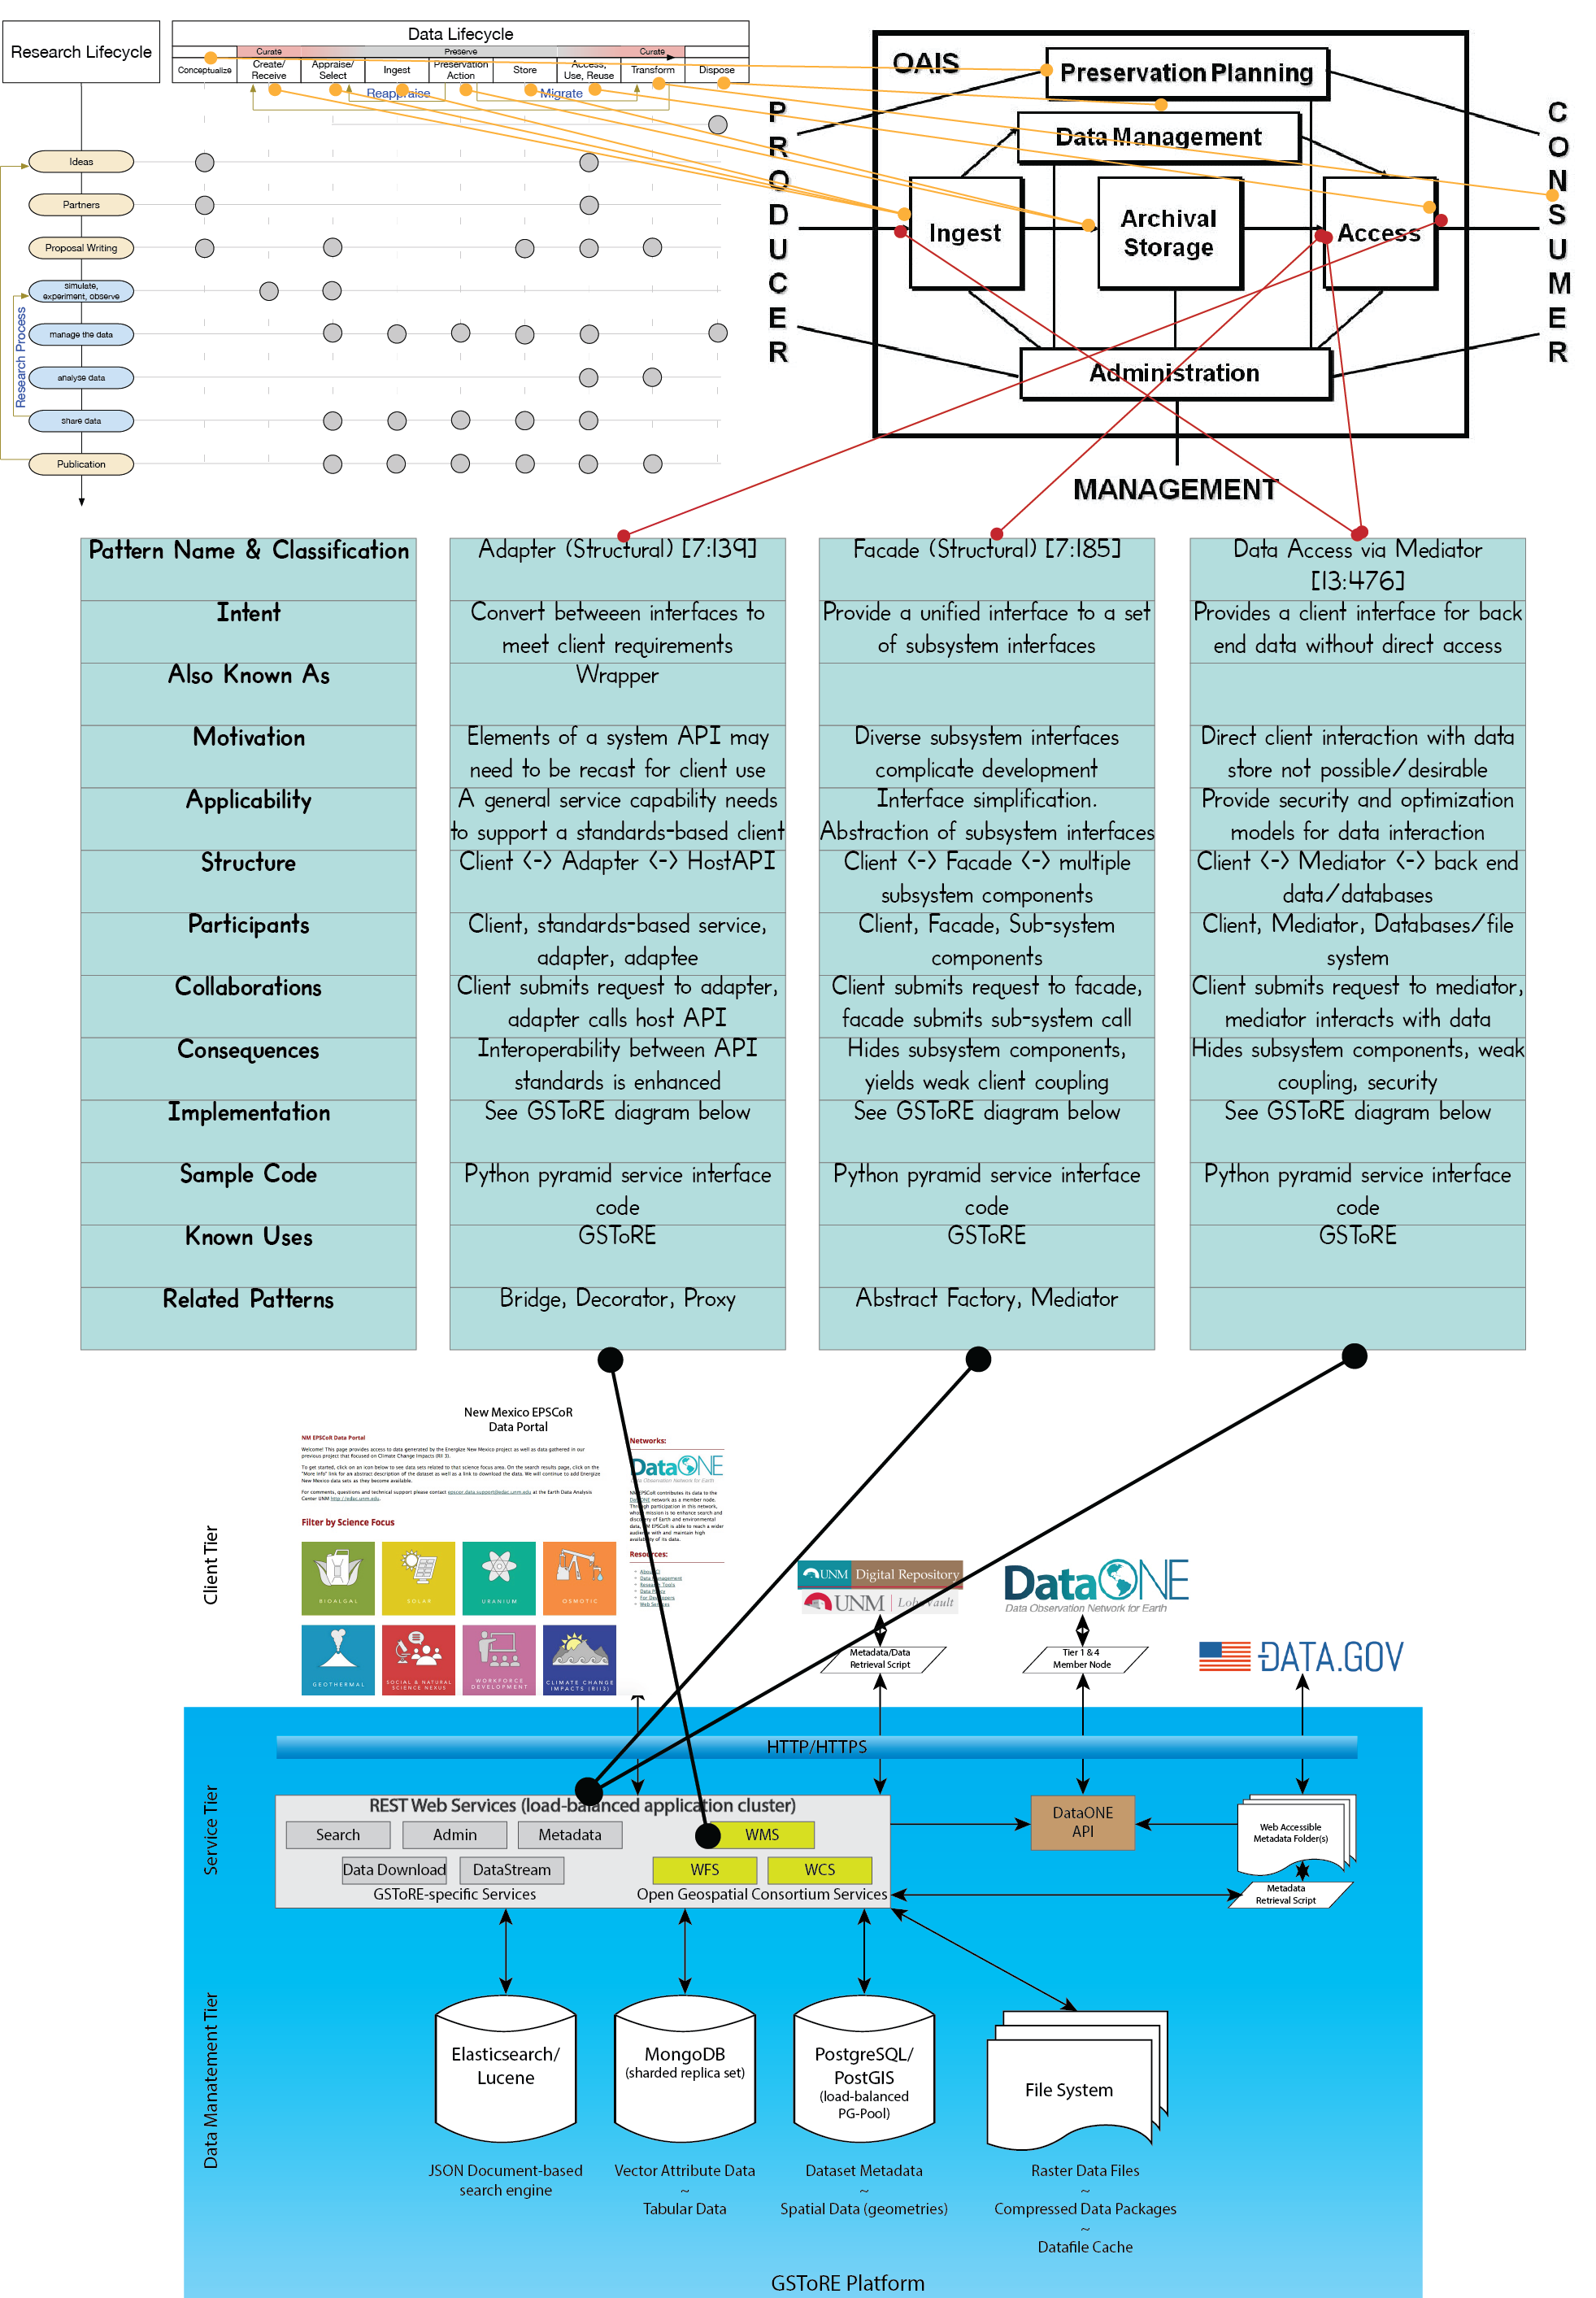
\includegraphics[width=11.00000in]{Composite-DesignPatternMapping.png}
\caption{Mapping of the GSToRE Platform's Capabilities into a Set of
Design Patterns and corresponding linkages between the OAIS Framework
and the Research Lifecycle}
\end{figure}

\section{Bibliography}\label{bibliography}

~

%==============================================================================
%==End of content==============================================================
%==============================================================================

\begin{footnotesize}


%--References------------------------------------------------------------------

\bibliography{2016-12_AGUPoster.bib}

%--End of references-----------------------------------------------------------

\end{footnotesize}

\end{multicols}

%==============================================================================
\end{frame}
\end{document}
